\documentclass[]{book}
\usepackage{lmodern}
\usepackage{amssymb,amsmath}
\usepackage{ifxetex,ifluatex}
\usepackage{fixltx2e} % provides \textsubscript
\ifnum 0\ifxetex 1\fi\ifluatex 1\fi=0 % if pdftex
  \usepackage[T1]{fontenc}
  \usepackage[utf8]{inputenc}
\else % if luatex or xelatex
  \ifxetex
    \usepackage{mathspec}
  \else
    \usepackage{fontspec}
  \fi
  \defaultfontfeatures{Ligatures=TeX,Scale=MatchLowercase}
\fi
% use upquote if available, for straight quotes in verbatim environments
\IfFileExists{upquote.sty}{\usepackage{upquote}}{}
% use microtype if available
\IfFileExists{microtype.sty}{%
\usepackage{microtype}
\UseMicrotypeSet[protrusion]{basicmath} % disable protrusion for tt fonts
}{}
\usepackage[margin=1in]{geometry}
\usepackage{hyperref}
\hypersetup{unicode=true,
            pdftitle={Package as Analysis},
            pdfauthor={Joshua H. Cook},
            pdfborder={0 0 0},
            breaklinks=true}
\urlstyle{same}  % don't use monospace font for urls
\usepackage{natbib}
\bibliographystyle{apalike}
\usepackage{color}
\usepackage{fancyvrb}
\newcommand{\VerbBar}{|}
\newcommand{\VERB}{\Verb[commandchars=\\\{\}]}
\DefineVerbatimEnvironment{Highlighting}{Verbatim}{commandchars=\\\{\}}
% Add ',fontsize=\small' for more characters per line
\usepackage{framed}
\definecolor{shadecolor}{RGB}{248,248,248}
\newenvironment{Shaded}{\begin{snugshade}}{\end{snugshade}}
\newcommand{\AlertTok}[1]{\textcolor[rgb]{0.94,0.16,0.16}{#1}}
\newcommand{\AnnotationTok}[1]{\textcolor[rgb]{0.56,0.35,0.01}{\textbf{\textit{#1}}}}
\newcommand{\AttributeTok}[1]{\textcolor[rgb]{0.77,0.63,0.00}{#1}}
\newcommand{\BaseNTok}[1]{\textcolor[rgb]{0.00,0.00,0.81}{#1}}
\newcommand{\BuiltInTok}[1]{#1}
\newcommand{\CharTok}[1]{\textcolor[rgb]{0.31,0.60,0.02}{#1}}
\newcommand{\CommentTok}[1]{\textcolor[rgb]{0.56,0.35,0.01}{\textit{#1}}}
\newcommand{\CommentVarTok}[1]{\textcolor[rgb]{0.56,0.35,0.01}{\textbf{\textit{#1}}}}
\newcommand{\ConstantTok}[1]{\textcolor[rgb]{0.00,0.00,0.00}{#1}}
\newcommand{\ControlFlowTok}[1]{\textcolor[rgb]{0.13,0.29,0.53}{\textbf{#1}}}
\newcommand{\DataTypeTok}[1]{\textcolor[rgb]{0.13,0.29,0.53}{#1}}
\newcommand{\DecValTok}[1]{\textcolor[rgb]{0.00,0.00,0.81}{#1}}
\newcommand{\DocumentationTok}[1]{\textcolor[rgb]{0.56,0.35,0.01}{\textbf{\textit{#1}}}}
\newcommand{\ErrorTok}[1]{\textcolor[rgb]{0.64,0.00,0.00}{\textbf{#1}}}
\newcommand{\ExtensionTok}[1]{#1}
\newcommand{\FloatTok}[1]{\textcolor[rgb]{0.00,0.00,0.81}{#1}}
\newcommand{\FunctionTok}[1]{\textcolor[rgb]{0.00,0.00,0.00}{#1}}
\newcommand{\ImportTok}[1]{#1}
\newcommand{\InformationTok}[1]{\textcolor[rgb]{0.56,0.35,0.01}{\textbf{\textit{#1}}}}
\newcommand{\KeywordTok}[1]{\textcolor[rgb]{0.13,0.29,0.53}{\textbf{#1}}}
\newcommand{\NormalTok}[1]{#1}
\newcommand{\OperatorTok}[1]{\textcolor[rgb]{0.81,0.36,0.00}{\textbf{#1}}}
\newcommand{\OtherTok}[1]{\textcolor[rgb]{0.56,0.35,0.01}{#1}}
\newcommand{\PreprocessorTok}[1]{\textcolor[rgb]{0.56,0.35,0.01}{\textit{#1}}}
\newcommand{\RegionMarkerTok}[1]{#1}
\newcommand{\SpecialCharTok}[1]{\textcolor[rgb]{0.00,0.00,0.00}{#1}}
\newcommand{\SpecialStringTok}[1]{\textcolor[rgb]{0.31,0.60,0.02}{#1}}
\newcommand{\StringTok}[1]{\textcolor[rgb]{0.31,0.60,0.02}{#1}}
\newcommand{\VariableTok}[1]{\textcolor[rgb]{0.00,0.00,0.00}{#1}}
\newcommand{\VerbatimStringTok}[1]{\textcolor[rgb]{0.31,0.60,0.02}{#1}}
\newcommand{\WarningTok}[1]{\textcolor[rgb]{0.56,0.35,0.01}{\textbf{\textit{#1}}}}
\usepackage{longtable,booktabs}
\usepackage{graphicx,grffile}
\makeatletter
\def\maxwidth{\ifdim\Gin@nat@width>\linewidth\linewidth\else\Gin@nat@width\fi}
\def\maxheight{\ifdim\Gin@nat@height>\textheight\textheight\else\Gin@nat@height\fi}
\makeatother
% Scale images if necessary, so that they will not overflow the page
% margins by default, and it is still possible to overwrite the defaults
% using explicit options in \includegraphics[width, height, ...]{}
\setkeys{Gin}{width=\maxwidth,height=\maxheight,keepaspectratio}
\IfFileExists{parskip.sty}{%
\usepackage{parskip}
}{% else
\setlength{\parindent}{0pt}
\setlength{\parskip}{6pt plus 2pt minus 1pt}
}
\setlength{\emergencystretch}{3em}  % prevent overfull lines
\providecommand{\tightlist}{%
  \setlength{\itemsep}{0pt}\setlength{\parskip}{0pt}}
\setcounter{secnumdepth}{5}
% Redefines (sub)paragraphs to behave more like sections
\ifx\paragraph\undefined\else
\let\oldparagraph\paragraph
\renewcommand{\paragraph}[1]{\oldparagraph{#1}\mbox{}}
\fi
\ifx\subparagraph\undefined\else
\let\oldsubparagraph\subparagraph
\renewcommand{\subparagraph}[1]{\oldsubparagraph{#1}\mbox{}}
\fi

%%% Use protect on footnotes to avoid problems with footnotes in titles
\let\rmarkdownfootnote\footnote%
\def\footnote{\protect\rmarkdownfootnote}

%%% Change title format to be more compact
\usepackage{titling}

% Create subtitle command for use in maketitle
\providecommand{\subtitle}[1]{
  \posttitle{
    \begin{center}\large#1\end{center}
    }
}

\setlength{\droptitle}{-2em}

  \title{Package as Analysis}
    \pretitle{\vspace{\droptitle}\centering\huge}
  \posttitle{\par}
    \author{Joshua H. Cook}
    \preauthor{\centering\large\emph}
  \postauthor{\par}
      \predate{\centering\large\emph}
  \postdate{\par}
    \date{2019-03-11}

\usepackage{booktabs}

\begin{document}
\maketitle

{
\setcounter{tocdepth}{1}
\tableofcontents
}
\hypertarget{welcome}{%
\chapter*{Welcome}\label{welcome}}
\addcontentsline{toc}{chapter}{Welcome}

This is a manual on how to use the standard R package framework for data analysis. Though potentially more work, especially at the start, the purpose of using the R package framework is to maintain a clear and reproducible analysis.

\textbf{{[}This book is currently in progress, though any \href{https://github.com/jhrcook/package-as-analysis/issues}{feedback} is welcome.{]}}

\hypertarget{why}{%
\subsection*{Why}\label{why}}
\addcontentsline{toc}{subsection}{Why}

Why bother with maintaining a package framework while also doing data analysis? It is a great question, especially when one considers the complexity and fluidity of an analysis and the rigidity of the R package framework. The answer is that some rigidity is needed - but just the basics. That is what the R package framework provides. There is a place for everything, though sometimes getting it to work (ie. build and pass checks) requires a few extra steps.

During my own analyses, I found things were getting much too disorganized and decentralized. What would start out as exploratory would morph into a subdirectory graph more complex than the oringinal parent analysis. Perhaps for more organized people, this is unnecessary, but for those of us who want order and aren't sure how to get it, this framework offers a great place to start.

The final (more abstract) reason for using the R package framework is to battle the current issue of reproducibility. Reproducibility is the cornerstone of science - if a finding it true, anyone should be able to replicate it. However, the scientific community has been dealing with an astounding amount of irreproducibility, most famously documented by the \href{http://science.sciencemag.org/content/349/6251/aac4716}{Open Science Collaboration}. If the analysis is organized as an R package, though, an analysis can be re-run entirely by anyone else familliar with R. Thus, whether they are collaborators and competitors, anyone should be able to follow the analysis a scientist publishes.

\hypertarget{advantages}{%
\subsection*{Advantages}\label{advantages}}
\addcontentsline{toc}{subsection}{Advantages}

There are many advantages to using this framework. Here are just a few, though I am sure you will find there are many others:

\begin{itemize}
\tightlist
\item
  Because this is a standard framework, other will be able to navigate the directories and files adeptly.
\item
  The implementation of tests on functions and subroutines will make bugs easier to find and increase overall confidence in the validity of the analysis
\item
  This is a seamless mixture of scripts and markdown files for the separation of functions and analysis
\item
  Complete documentation of functions makes returning to code later much easier!
\item
  The analysis can take advantage of normal R package tools such as \href{https://travis-ci.org}{Travis-CI} and \href{https://codecov.io}{Codecov} integration, \href{https://pkgdown.r-lib.org}{pkgdown}, and \href{https://devtools.r-lib.org}{devtools} (build checks, documentation, etc.).
\end{itemize}

\hypertarget{examples}{%
\subsection*{Examples}\label{examples}}
\addcontentsline{toc}{subsection}{Examples}

{[}coming soon{]} Allele-specific \emph{KRAS} copy number alteration

\hypertarget{about}{%
\section*{About}\label{about}}
\addcontentsline{toc}{section}{About}

\hypertarget{about-this-book}{%
\subsection*{About this Book}\label{about-this-book}}
\addcontentsline{toc}{subsection}{About this Book}

{[}TODO{]}

\hypertarget{about-the-author}{%
\subsection*{About the Author}\label{about-the-author}}
\addcontentsline{toc}{subsection}{About the Author}

I am a classically-trained biologist-turned computational biologist. I graduated with degrees in Molecular Biology and Biochemistry, and Chemistry from the University of California, Irvine in 2017. My research focused on investigating the patterns and mechanisms of dissemination by which \emph{Toxoplasma gondii}, an obligate, intracellular parasite, infects a human host \href{https://www.ncbi.nlm.nih.gov/pubmed/29295815}{Cook \emph{et al.}, 2018}. I started my graduate studies at Harvard Medical School in 2018, and after rotating in a chemical biology lab and a \emph{Vibrio cholerae} lab, I finally decided to study cancer using computational biology. Since then, and continuing still today, I have been learning computer programming and statistics, trying to catch up to my peers. Consequently, I have fallen in love with R, especially because of the \href{https://www.tidyverse.org}{Tyidyverse} and tidy data.

\hypertarget{resources}{%
\section*{Resources}\label{resources}}
\addcontentsline{toc}{section}{Resources}

The best resource for making R packages is \href{http://r-pkgs.had.co.nz}{R Packages} by Hadley Wickham.

There are some useful R packages you will want to have installed:

\begin{itemize}
\tightlist
\item
  \texttt{devtools} - will do most of the development building and checking
\item
  \texttt{roxygen2} - makes all of the documentation
\item
  \texttt{usethis} - for preparing all of the pieces and tools you want to include
\item
  \texttt{testthat} - for running tests
\item
  \texttt{kintr} - for compiling all of the Rmarkdown files
\end{itemize}

These can be installed using the following code.

\begin{Shaded}
\begin{Highlighting}[]
\KeywordTok{install.packages}\NormalTok{(}\KeywordTok{c}\NormalTok{(}\StringTok{"devtools"}\NormalTok{, }\StringTok{"roxygen2"}\NormalTok{, }\StringTok{"usethis"}\NormalTok{, }\StringTok{"testthat"}\NormalTok{, }\StringTok{"knitr"}\NormalTok{))}
\end{Highlighting}
\end{Shaded}

\hypertarget{license}{%
\section*{License}\label{license}}
\addcontentsline{toc}{section}{License}

This work is under a \href{http://creativecommons.org/licenses/by-nc-sa/4.0/}{Attribution-NonCommercial-ShareAlike 4.0 International License (CC BY-NC-SA 4.0)}

\hypertarget{framework}{%
\chapter{Framework}\label{framework}}

\hypertarget{introduction}{%
\section{Introduction}\label{introduction}}

I have decided to introduce the R packagge framework before going through the set-up process because, quite frankly, I think this is more important. There are many sites that outline the steps of creating an R package (they likely do it better than I will next chapter), but the main point of this book is how to make the R package into a data analysis project. Therfore, understanding the use of the framework should be the reader's focus, here.

I try to adhere to the following process for each peace of the framework:

\begin{enumerate}
\def\labelenumi{\arabic{enumi}.}
\tightlist
\item
  what is it and what is its main role?
\item
  when does it need to be used or adjusted?
\item
  what is unique about its use for a data analysis project?
\end{enumerate}

{[}TODO{]}

Include a subsetion on each main peice of package:

\begin{itemize}
\tightlist
\item
  what is it for
\item
  things to be wary of
\item
  specific use for data analysis
\end{itemize}

\hypertarget{getting-started}{%
\chapter{Getting Started}\label{getting-started}}

Setting up the package is mostly automated and is well documented in \href{http://r-pkgs.had.co.nz/intro.html}{R Packages} by Hadley Wickham. If you are running the analysis on your local machine, I would recommend using \href{https://www.rstudio.com}{RStudio} (which you likely already do), but this is possible to do on a remote computing cluster (which is how I work). I begin by going through the steps of setting up the basic package framework, which is the same for local or remote work. Following that, there is a section for how I work remotely. This can be skipped if you only work locally or if you already have a system you enjoy (though I highly recommend the system I currently use). I finish off with a few extras that I recommend using, but are not necessary.

\hypertarget{r-package-set-up}{%
\section{R Package Set Up}\label{r-package-set-up}}

The set up process is rather simple. If using RStudio, you can start a new R project as a package. Otherwise, the following command will get the basic framework started. There is a lot of overlap between the devtools and usethis package. I believe that RStudio is trying to fade out devtools and instead have people use the various packages that were split from it, including usethis.

The advantage to using the usethis functions for seemingly simple tasks (such as making the ``data-raw'' directory) is that it will also add the necessary lines to ``.RBuildignore,'' the ``DESCRIPTION,'' and ``NAMESPACE'' if needed.

It's easy to create the package from the R console.

\begin{Shaded}
\begin{Highlighting}[]
\NormalTok{usethis}\OperatorTok{::}\KeywordTok{create}\NormalTok{(}\StringTok{"path/to/package/pkgname"}\NormalTok{)}
\end{Highlighting}
\end{Shaded}

You can then add a license as shown below. I generally use a GPL-3, though you can get a lot of information on the common licenses at \href{https://choosealicense.com}{choosealicense.com}.

\begin{Shaded}
\begin{Highlighting}[]
\NormalTok{usethis}\OperatorTok{::}\KeywordTok{use_gpl3_license}\NormalTok{(}\DataTypeTok{name =} \StringTok{"Your Name"}\NormalTok{)}
\end{Highlighting}
\end{Shaded}

Prepare the project to use roxygen for documentation.

\begin{Shaded}
\begin{Highlighting}[]
\NormalTok{usethis}\OperatorTok{::}\KeywordTok{use_roxygen_md}\NormalTok{()}
\end{Highlighting}
\end{Shaded}

Create a README file. You can also opt to use a normal Markdown file with \texttt{usethis::use\_readme\_md()}, though I would recommend to just go with an RMarkdown file.

\begin{Shaded}
\begin{Highlighting}[]
\NormalTok{usethis}\OperatorTok{::}\KeywordTok{use_readme_rmd}\NormalTok{()}
\end{Highlighting}
\end{Shaded}

Create a ``NEWS'' file for announcing major changes to the project.

\begin{Shaded}
\begin{Highlighting}[]
\NormalTok{usethis}\OperatorTok{::}\KeywordTok{use_news_md}\NormalTok{()}
\end{Highlighting}
\end{Shaded}

Create a ``data-raw'' directory.

\begin{Shaded}
\begin{Highlighting}[]
\NormalTok{usethis}\OperatorTok{::}\KeywordTok{use_data_raw}\NormalTok{()}
\end{Highlighting}
\end{Shaded}

Finally, set up the use of testthat package for testing.

\begin{Shaded}
\begin{Highlighting}[]
\NormalTok{usethis}\OperatorTok{::}\KeywordTok{use_testthat}\NormalTok{()}
\end{Highlighting}
\end{Shaded}

\textbf{Note:} If you are working remotely (ie. sshing to the computer running the code), many of the usethis functions will open the file that you just asked them to create (eg. open ``NEWS.md'' after using \texttt{use\_news\_md()}) in vim. To suppress this, just pass the paramter \texttt{open\ =\ FALSE}. Otherwise, it is set to \texttt{interactive()}.

\hypertarget{git-and-github}{%
\subsection{Git and GitHub}\label{git-and-github}}

If you are programming, you should be using git. This is especially important in the sciences because git logs can be used to resolve legal conflicts and issues of data falsification. GitHub is not essential, though I would highly recommend you use it because it makes managing files and collaboration much easier. It is also essential for taking advantage of some of the best parts of an R package such as build checks and \texttt{pkgdown} (see Extras below)

To get started with git, there are \emph{tons} of resources available, so I will not describe it here. If you are new to git and GitHub, here are a few good resources to get you started:

\begin{itemize}
\tightlist
\item
  \href{https://medium.freecodecamp.org/what-is-git-and-how-to-use-it-c341b049ae61}{An introduction to Git: what it is, and how to use it}
\item
  \href{https://www.digitalocean.com/community/tutorials/how-to-use-git-a-reference-guide}{How To Use Git: A Reference Guide}
\item
  \href{https://guides.github.com/activities/hello-world/}{GitHub Guides: Hello World}
\end{itemize}

There is a usethis function to initiate git (\texttt{usethis::use\_git()}) though I always prefer to set up myself.

\hypertarget{remote}{%
\section{Remote}\label{remote}}

If you conduct work remotely, I'm going to assume that you have ssh set up and running. Otherwise, there are plenty of resources available, and you should review the material available by your system admin.

Though I prefer Rstudio for normal package development, I spare my computer the pain of performing complex and heavy computation, opting instead to off-load it to the \href{https://rc.hms.harvard.edu}{Harvard Medical School Research Computing Cluster}. Therefore, I use \href{https://www.sublimetext.com}{SublimeText3} as by text editor and send code to the remote comuting node over ssh using \href{https://iterm2colorschemes.com}{iTerm2} as my terrminal. Finally, I use SSH File System (SSHFS) to ``mount'' the remote directory to my local directory.

\hypertarget{sublimetext3-set-up}{%
\subsection{SublimeText3 Set-Up}\label{sublimetext3-set-up}}

Here are the handful of SublimeText3 (ST3) packages I use for R coding, followed by any particular notes on their use:

\begin{itemize}
\tightlist
\item
  \href{https://packagecontrol.io/packages/LSP}{LSP} - ``Gives Sublime Text 3 rich editing features for languages with Language Server Protocol support''
\item
  \href{https://packagecontrol.io/packages/MarkdownEditing}{MarkdownEditing} - ``Markdown plugin for Sublime Text. Provides\ldots{} more robust syntax highlighting and useful Markdown editing features for Sublime Text.''
\item
  \href{https://packagecontrol.io/packages/R-IDE}{R-IDE} - ``{[}A{]}iming to utilize the use of language server + better support R Markdown + better support of R packaging + \ldots{}''
\item
  \href{https://packagecontrol.io/packages/SendCode}{SendCode} - ``Send code and text to macOS and Linux Terminals, iTerm, ConEmu, Cmder, Tmux, Terminus; R (RStudio), Julia, IPython.''
\end{itemize}

LSP and R-IDE handle syntax and completion in ST3. It isn't a great system, so if you know of a better set-up in ST3, \href{https://github.com/jhrcook/package-as-analysis/issues}{please let me know}. MarkdownEditing and R-IDE combine to make RMarkdown feasible. The SendCode package essentially copies, pastes, and runs my code written in ST3 to the terminal when I press \texttt{command} + \texttt{return}. This way, I can type in ST3 and run in the terminal without using the mouse.

Before moving on, I made this snippet to quickly add a code chunk.

\begin{Shaded}
\begin{Highlighting}[]
\KeywordTok{<snippet>}
        \KeywordTok{<content>}\BaseNTok{<![CDATA[}
\NormalTok{```\{r $\{1:chunk_name\}\}}
\NormalTok{$0}
\NormalTok{```}
\BaseNTok{]]>}\KeywordTok{</content>}
        \CommentTok{<!-- Optional: Set a tabTrigger to define how to trigger the snippet -->}
        \KeywordTok{<tabTrigger>}\NormalTok{rchunk}\KeywordTok{</tabTrigger>}
        \CommentTok{<!-- Optional: Set a scope to limit where the snippet will trigger -->}
        \KeywordTok{<scope>}\NormalTok{text.html.markdown.multimarkdown, text.html.markdown}\KeywordTok{</scope>}
        \KeywordTok{<description>}\NormalTok{create a Rmd code chunk}\KeywordTok{</description>}
\KeywordTok{</snippet>}
\end{Highlighting}
\end{Shaded}

\hypertarget{using-ssh-file-system}{%
\subsection{Using SSH File System}\label{using-ssh-file-system}}

I use SSH File System (SSFHS) to ``mount'' my remote directory to my local directory. It is essentually SFTP and SSH combined (the details go right over my head) and it is fairly easy to get set-up. Here is a \href{https://github.com/osxfuse/osxfuse/wiki/SSHFS}{link} to get everything going, and I have included the steps I used below.

To start I downloaded and installed \href{https://osxfuse.github.io}{FUSE for macOS}. Then I downloaded and installed the \href{https://github.com/osxfuse/sshfs/releases}{latest build of SSHFS}. Finally, I created an empty directory that will become the place that I mount the remote directory. Typically, I make the root of the package, though I could see instances where you would want the package in a subdirectory below it.

\begin{Shaded}
\begin{Highlighting}[]
\CommentTok{# on local}
\FunctionTok{mkdir}\NormalTok{ ~/Lab_Projects/pkgName}
\end{Highlighting}
\end{Shaded}

On the remote server, I make a directory with the same name

\begin{Shaded}
\begin{Highlighting}[]
\CommentTok{# on remote}
\ExtensionTok{/path/to/compute/directory/pkgName}
\end{Highlighting}
\end{Shaded}

Finally, to connect the two, I use the following command that is pretty much identical to initiating a normal ssh session.

\begin{Shaded}
\begin{Highlighting}[]
\CommentTok{# on local}
\ExtensionTok{sshfs}\NormalTok{ username@remote.host.com:/path/to/compute/directory/pkgName ~/Lab_Projects/pkgName}
\end{Highlighting}
\end{Shaded}

Now, the computer will treat the mount just like a normal flash drive, and ST3 fully accepts it. The only change I made to ST3 was to map a key-binding to ``Project/Refresh Folders''. This way, if new files are created remotely, a quick key-stroke and everything is visible in the ST3 sidebar.

\hypertarget{git-and-github-1}{%
\subsection{Git and GitHub}\label{git-and-github-1}}

If working remotely, I have found it much easier to handle everything git-related on the remote side. Therefore, I created ssh RSA keys and shared the public one with the GitHub repo so I could push over ssh. Setting this up is pretty simple and well outlined in \href{https://help.github.com/en/articles/connecting-to-github-with-ssh}{Connecting to GitHub with SSH}.

\hypertarget{extras}{%
\section{Extras}\label{extras}}

Though these next few items are not required, I \emph{highly recommend} implementing them because they each take advantage of the fact that this project adheres to the standard R framework. Their different functions are all reasons to go through the trouble of mainting this framework.

\hypertarget{pkgdown}{%
\subsection{pkgdown}\label{pkgdown}}

Pkgdown ties a bow around your package, slaps it on the bottom, and builds a gorgeous and professional website rich with useful features. It builds the documentation for easy reference, presents the vignettes, and organizes all of the package meta-data so it is easily viewable and understandable. Here are some packages that take advantage of pkgdown:

\begin{itemize}
\tightlist
\item
  \href{https://pkgdown.r-lib.org}{pkgdown} (of course)
\item
  \href{https://ggplot2.tidyverse.org}{ggplot2}
\item
  \href{https://nanx.me/ggsci/}{ggsci}
\item
  \href{https://jhrcook.github.io/ggasym/index.html}{ggasym} (a shameless plug of my own lil' package)
\end{itemize}

The use of pkgdown obviously begins with a usethis function.

\begin{Shaded}
\begin{Highlighting}[]
\NormalTok{usethis}\OperatorTok{::}\KeywordTok{use_pkgdown}\NormalTok{()}
\end{Highlighting}
\end{Shaded}

All that you have to do from there is use \texttt{pkgdown::build\_site()} to build the site whenever the project is at a good stopping point for the day. (If working remotely, pass \texttt{preview\ =\ FALSE} to prevent pkgdown from searching for a browser to display in when completed.)

To show the website on GitHub, go to ``Settings'' in the repository, and select ``master branch /docs folder'' from the options in the ``GitHub Pages'' section. It should look something like this (another shameless plug for lil' ole' ggasym).

\begin{Shaded}
\begin{Highlighting}[]
\NormalTok{knitr}\OperatorTok{::}\KeywordTok{include_graphics}\NormalTok{(}\StringTok{"images/github-pages.png"}\NormalTok{)}
\end{Highlighting}
\end{Shaded}

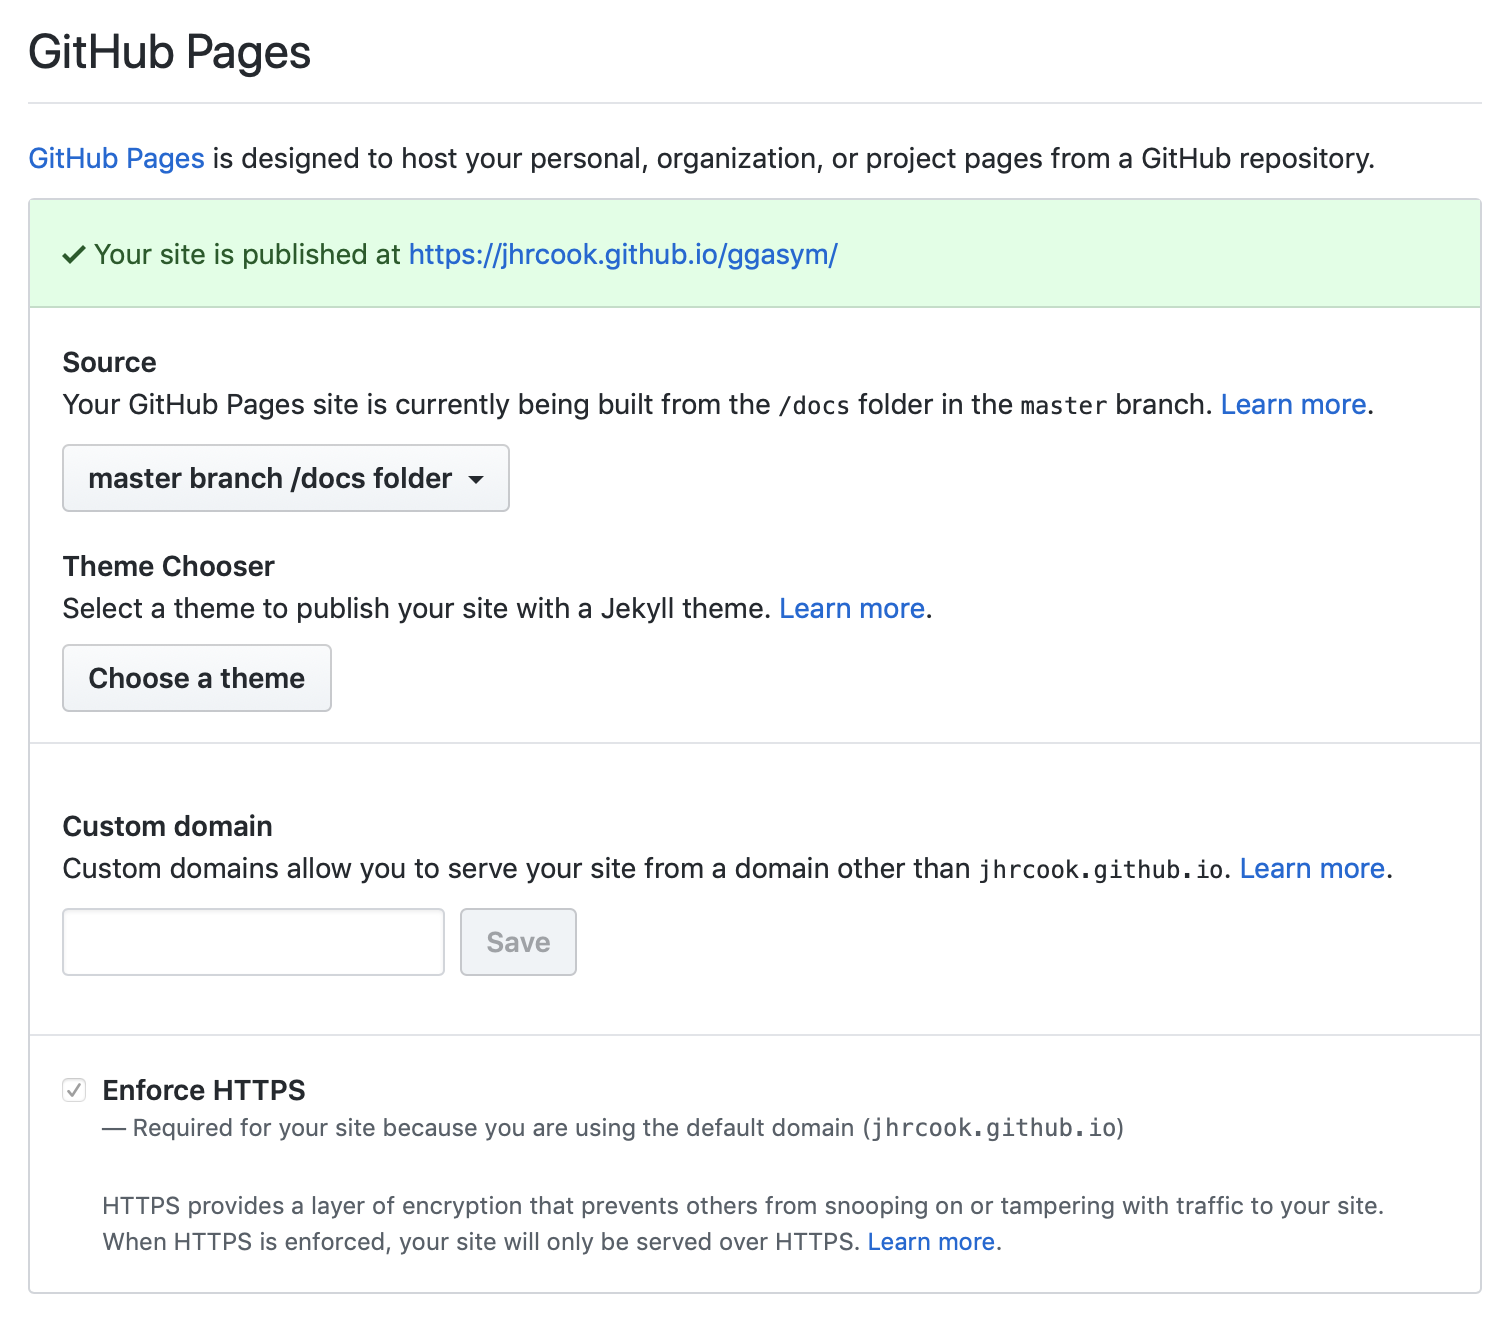
\includegraphics[width=20.97in]{images/github-pages}

\hypertarget{travis-ci-appveyor-and-codecov}{%
\subsection{Travis-CI, Appveyor, and Codecov}\label{travis-ci-appveyor-and-codecov}}

GitHub integration also opens up the use of continuous integration (CI) apps. \href{https://travis-ci.org}{Travis-CI} and \href{https://www.appveyor.com}{Appveyor} are useful for checking the build status of the package. I just use both because they each require so little effort to integrate and each provides their own suite of functions. Noteably, Appveyor build the package on Linux and Windows. To get started, just use usethis.

\href{https://codecov.io}{Codecov} provides an indication as to how well the package's tests cover the code. Though not a perfect measure of test quality (nothing ever will be), I find this tool to be helpful for me to find which functions I have and have not created tests for.

\begin{Shaded}
\begin{Highlighting}[]
\NormalTok{usethis}\OperatorTok{::}\KeywordTok{use_travis}\NormalTok{()}
\NormalTok{usethis}\OperatorTok{::}\KeywordTok{use_coverage}\NormalTok{(}\StringTok{"codecov"}\NormalTok{)}
\NormalTok{usethis}\OperatorTok{::}\KeywordTok{use_appveyor}\NormalTok{()}
\end{Highlighting}
\end{Shaded}

You then just follow the instructions printed out to get everything set up. If this your first time useing any of the tools, then you will have to grant them access to your GitHub repositories, and they will do the rest.

The usethis command will also procuce the markdown code for showing the status badges for each tools. Placing these below the package name in the README.Rmd is sstandard practice and will tell pkgdown to put them in the side bar of the site.

On top of looking good and being informative for you during the development process, these badges will also provide visitors an indication as to the quality and maintaince of the package. A few good badges will likely make visitors more trusting of your results.

\hypertarget{spelling}{%
\subsection{Spelling}\label{spelling}}

TODO

\hypertarget{workflow}{%
\chapter{Workflow}\label{workflow}}

\hypertarget{example-allele-specific-kras-cna}{%
\chapter{\texorpdfstring{Example: Allele-specific \emph{KRAS} CNA}{Example: Allele-specific KRAS CNA}}\label{example-allele-specific-kras-cna}}

{[}in progress{]}

\bibliography{book.bib}


\end{document}
